\subsection{bpmdsp/discrete\_\-fourier\_\-transforms.c File Reference}
\label{discrete__fourier__transforms_8c}\index{bpmdsp/discrete\_\-fourier\_\-transforms.c@{bpmdsp/discrete\_\-fourier\_\-transforms.c}}


\subsubsection{Detailed Description}


Definition in file {\bf discrete\_\-fourier\_\-transforms.c}.

{\tt \#include \char`\"{}bpm/bpm\_\-wf.h\char`\"{}}\par
{\tt \#include \char`\"{}bpm/bpm\_\-dsp.h\char`\"{}}\par


Include dependency graph for discrete\_\-fourier\_\-transforms.c:\nopagebreak
\begin{figure}[H]
\begin{center}
\leavevmode
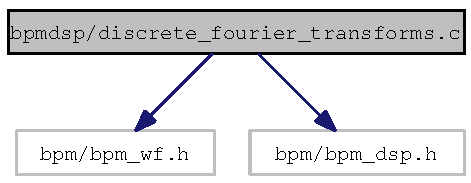
\includegraphics[width=131pt]{discrete__fourier__transforms_8c__incl}
\end{center}
\end{figure}
\subsubsection*{Functions}
\begin{CompactItemize}
\item 
void \textbf{cdft} (int, int, double $\ast$, int $\ast$, double $\ast$)\label{discrete__fourier__transforms_8c_dd439be0f19853cd7568299e4e9f2043}

\item 
void \textbf{rdft} (int, int, double $\ast$, int $\ast$, double $\ast$)\label{discrete__fourier__transforms_8c_39caf6956db3e0243c1a29009d4bf68c}

\item 
int \textbf{\_\-is\_\-pow2} (int n)\label{discrete__fourier__transforms_8c_ae95d6a6ef87ec161047540b4e675fdd}

\item 
int \textbf{\_\-check\_\-fft\_\-buffers} (int ns)\label{discrete__fourier__transforms_8c_fa13ee764b0fe25cf3c4b99e5205bb5d}

\item 
int {\bf fft\_\-gen\_\-tables} (void)
\item 
int {\bf fft\_\-initialise} (int ns)
\item 
void {\bf fft\_\-cleanup} (void)
\item 
int {\bf complexfft} ({\bf complexwf\_\-t} $\ast$z, int fft\_\-mode)
\item 
int {\bf realfft} ({\bf doublewf\_\-t} $\ast$y, int fft\_\-mode, {\bf complexwf\_\-t} $\ast$z)
\end{CompactItemize}
